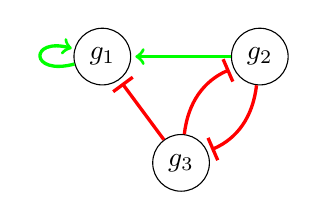
\begin{tikzpicture}[scale=0.5]
	\path(0,0)    node[draw, fill=white!20,shape=circle](G1) {$g_1$};
	\path(4,0)    node[draw, fill=white!20,shape=circle](G2) {$g_2$};
	\path(2,-2.7) node[draw, fill=white!20,shape=circle](G3) {$g_3$};
	\draw[->, thick] (G1) edge[very thick,green, loop left] (G1);
	\draw[->, thick] (G2) edge[very thick,green,shorten >=1.5pt] (G1);
	\draw[-|, thick,shorten >=1.5pt] (G3) edge[very thick,red] (G1);
	\draw[-|, thick,shorten >=1.5pt] (G3) edge[very thick,red, bend left=30] (G2);
	\draw[-|, thick,shorten >=1.5pt] (G2) edge[very thick,red, bend left=30] (G3);
\end{tikzpicture}

